\documentclass[../main.tex]{subfiles}

\begin{document}

\chapter{Related work}
One of the first applications of \emph{graph theory} was when \emph{Leonhard Euler} considered the \emph{Königsberg bridge problem}: Is there a way to walk over the seven bridges of Königsberg only once?

It is trivial to see that there is a close correlation between graphs and maps, as you can see in figure \ref{fig:road_graph}, with the roads and junctions in the map being lines and dots in the graph.  A line is mostly called \textit{edge} or \textit{arc} and a connecting dot is called \textit{vertex}, \textit{node} or \textit{point}; in this report it will mostly be \textit{vertex} and \textit{edge}, but to differentiate, another type of graphs called \textit{line graph} will use the names \textit{node} and \textit{line} to distinguish. As one delves deeper into the theoretical material, one will find that there is good to know some \emph{graph theory} and be familiar with some definitions.

\begin{figure}[h]
\centering
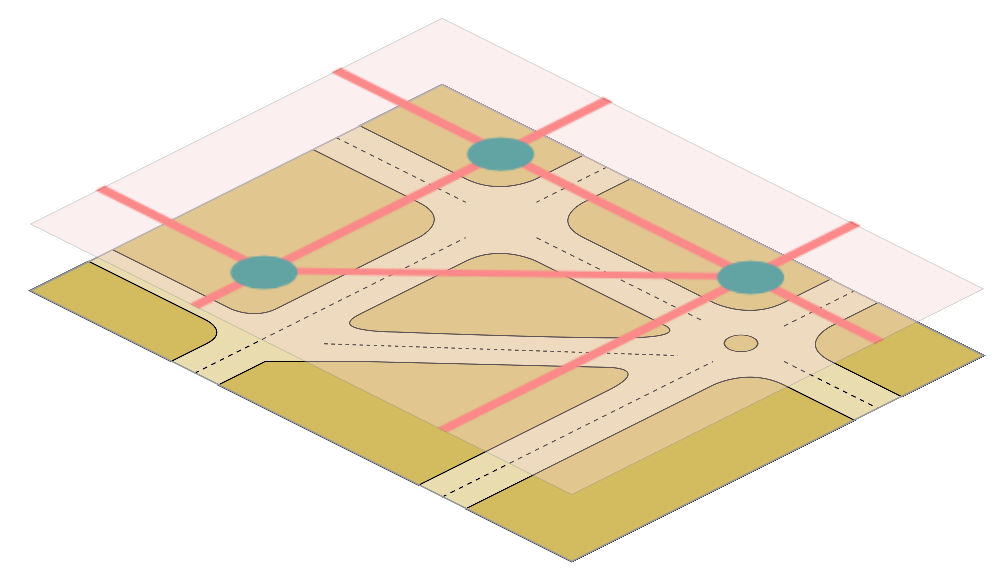
\includegraphics[width=0.7\textwidth]{road_graph_iso}
\caption{Graphs and road maps are a natural match.}
\label{fig:road_graph}
\end{figure}

\section{Graph theory}
There are good lecture notes such those from \emph{Tampere University of Technology} \cite{ruohonen-graph-theory} and \emph{Univerity of Turku} \cite{harju-graph-theory} (both happen to be Finnish) and a good text book by \emph{Reinhard Diestel} \cite{diestel} are available to get into this subject. One does not need to understand all the concepts, but be familiar with some basic definitions and notations.

A \textit{graph} is made up by \textit{vertices} and \textit{edges}, see figure \ref{fig:edge_vertex_graph}.

\begin{figure}[h]
    \centering
    \begin{subfigure}[Undirected]{0.4\linewidth}
        \centering
        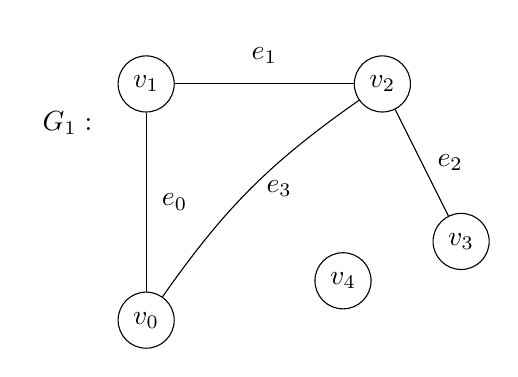
\begin{tikzpicture}
            \tikzstyle{every node} = [draw, shape=circle]
            \tikzstyle{ann} = [draw=none, fill=none]
            \node (v0) at (0,0) {$v_0$};
            \node (v1) at (0,3) {$v_1$};
            \node (v2) at (3,3) {$v_2$};
            \node (v3) at (4,1) {$v_3$};
            \node (v4) at (2.5,0.5) {$v_4$};
            \draw (v0) edge node[ann,right] {$e_0$} (v1);
            \draw (v1) edge node[ann,above] {$e_1$} (v2);
            \draw (v2) edge node[ann,right] {$e_2$} (v3);
            \draw (v2) edge[bend right=10] node[ann,right] {$e_3$} (v0);
            \node[ann] at (-1,2.5) {$G_1:$};
        \end{tikzpicture}
        \caption{Undirected}
        \label{fig:edge_vertex_graph_a}
    \end{subfigure}
    \hspace{5mm}
    \begin{subfigure}[Directed]{0.4\linewidth}
        \centering
        \begin{tikzpicture}
            \tikzstyle{every node} = [draw, shape=circle]
            \tikzstyle{ann} = [draw=none, fill=none]
            \node (v0) at (0,0) {$v_0$};
            \node (v1) at (0,3) {$v_1$};
            \node (v2) at (3,3) {$v_2$};
            \node (v3) at (4,1) {$v_3$};
            \draw[-Latex] (v0) edge[bend right=10] node[ann,right] {$e_0$} (v1);
            \draw[-Latex] (v1) edge node[ann,above] {$e_1$} (v2);
            \draw[-Latex] (v2) edge node[ann,right] {$e_2$} (v3);
            \draw[-Latex] (v2) edge[bend right=10] node[ann,right] {$e_3$} (v0);
            \draw[-Latex] (v1) edge[bend right=10] node[ann,left] {$e_4$} (v0);
            \node[ann] at (-1,2.5) {$G_2:$};
        \end{tikzpicture}
        \caption{Directed}
        \label{fig:edge_vertex_graph_b}
    \end{subfigure}
    \caption{A \textit{graph} with \textit{vertices} and \textit{edges}.}
    \label{fig:edge_vertex_graph}
\end{figure}

So a graph $G$ is a pair of sets, $G = (V,E)$ where $V=\{v_0, ...\}$ is the set of vertices and $E=\{e_0, ...\}$ is the set of edges. The edges can have their own labels as in the figure, or they can be denoted by the pair of vertices they connect: $e_0$ could be also named as $(v_0,v_1)$ or $v_0v_1$. A graph can be \emph{undirected} (figure \ref{fig:edge_vertex_graph_a}) if the edges have no sense of direction, or it can be \emph{directed} (figure \ref{fig:edge_vertex_graph_b}) if the direction of travel along an edge matters; $e_0$ is distinct from $e_4$ because the have different directions although they connect the same nodes $v_0$ and $v_1$. A directed graph can also be called a \emph{digraph}.

To decide how ``big'' a graph is, one can count the number of vertices, $|V|$, to get the \emph{order} or \emph{cardinality} of the graph. If one counts the number of edges, $|E|$ one gets the \emph{size} of the graph. In figure \ref{fig:edge_vertex_graph}, $G_1$ has order 5, and size 4; and $G_2$ has order 4 and size 5.

Edges are \emph{adjacent} if they share a common vertex, and vertices are adjacent if they are connected by an edge, one can also say that $v$ is \emph{incident} with $e$. In figure \ref{fig:edge_vertex_graph_a}, $v_0$ and $v_1$ are adjacent but not $v_1$ and $v_3$, and $e_0$ and $e_1$ are adjacent but not $e_0$ and $e_2$. 

The number of edges connecting to a vertex is called the \emph{degree} of the vertex, $d(v)$. In figure \ref{fig:edge_vertex_graph_a}, $d(v_2) = 3$, $d(v_3) = 1$ and $d(v_4) = 0$. A vertex of degree 1 is called a \emph{pendant} vertex, or \emph{leaf}, and a vertex of degree 0 is called \emph{isolated}. If all \emph{components} of a graph are \emph{connected}, then the graph is a connected graph. In figure \ref{fig:edge_vertex_graph} graph $G_2$ is connected, but graph $G_1$ is not because it has an isolated vertex as a component.

A graph is \emph{planar} if it is possible to draw without edges crossing each other. It is \emph{Eulerian} if one can travel over every edge in the graph only once (as in the \emph{Königsberg bridge problem}). A graph is called \emph{Hamiltonian} if one can visit every vertex in the graph only once (as in the \emph{Travelling salesman problem}).

Travels in graphs can be called different names. Ruohonen \cite{ruohonen-graph-theory} has the most general name \emph{walk} for travel from vertex to vertex along edges. A walk is \emph{open} if it ends on a different vertex than it started, or \emph{closed} if it ends on the same vertex. If an edge is traversed only once, the walk is called a \emph{trail}. If any vertex is visited only once then the trail is a \emph{path}. If the walk is a path but with the start and ending vertices being the same, then the walk is a \emph{circuit}.

One can partition a graph into \emph{subgraphs} if on places a cut in a vertex (\emph{cut vertex}) or over a set of edges (\emph{cut set}). In figure \ref{fig:edge_vertex_graph_a} a cut vertex could be $v_2$ and a cut set could be $\{e_1, e_3\}$.


\subsection{Graph representation} \label{graph_representations}
There are different ways of representing graphs. We have so far used

\begin{itemize}
\item Graph diagram
\item Set definitions, $V(G)=\{v_0,v_1,v_2,v_3,...\}, \quad E(G)=\{e_0,e_1,e_2,e_3,...\}$ 
\end{itemize}

One can also use
\begin{itemize}
\item \emph{Adjacency matrix}
\item \emph{Incidence matrix}
\item \emph{Adjacency list}
\end{itemize}

An \emph{adjacency matrix} is a matrix that shows if vertices are adjacent or not. A value of $0$ indicates that the vertices are not adjacent. For an \emph{unweighted} graph, adjacency can be indicated with a $1$, or if it is a \emph{weighted graph}, it can be the value of the weight (e.g. edge length or cost). From figure \ref{fig:edge_vertex_graph_a}:

\kbalignrighttrue
\renewcommand{\kbldelim}{(}% Left delimiter
\renewcommand{\kbrdelim}{)}% Right delimiter
% \[
\begin{equation}
  D = \kbordermatrix{
    & v_0 & v_1 & v_2 & v_3 & v_4 \\
    v_0 & 0 & 1 & 1 & 0 & 0 \\
    v_1 & 1 & 0 & 1 & 0 & 0 \\
    v_2 & 1 & 1 & 0 & 1 & 0 \\
    v_3 & 0 & 0 & 1 & 0 & 0 \\
    v_4 & 0 & 0 & 0 & 0 & 0
  }
% \]
\end{equation}

\vspace{1em}
\noindent
An \emph{incidence matrix} describes which vertices that are incident with which edges. In a directed graph it is \emph{positive} if it is the \emph{start} vertex of the edge, or \emph{negative} if it is the \emph{ending} vertex of the edge. From figure \ref{fig:edge_vertex_graph_b}:

\kbalignrighttrue
\renewcommand{\kbldelim}{(}% Left delimiter
\renewcommand{\kbrdelim}{)}% Right delimiter
% \[
\begin{equation}
  A = \kbordermatrix{
    & e_0 & e_1 & e_2 & e_3 & e_4 \\
    v_0 & 1 & 0 & 0 & -1 & -1 \\
    v_1 & -1 & 1 & 0 & 0 & 1 \\
    v_2 & 0 & -1 & 1 & 1 & 0 \\
    v_3 & 0 & 0 & -1 & 0 & 0
  }
% \]
\end{equation}

\vspace{1em}
\noindent
A \emph{dense} graph has almost all vertices connected to each other, i.e. there are few $0$s in the adjacency matrix. In a \emph{sparse} graph there are a lot fewer edges than there could be, so the adjacency matrix has a lot of $0$s. To be space efficient, especially in computing, it can therefore be better to represent a graph as an \emph{adjacency list}, which simply lists for each vertex which other vertices it is adjacent to. No $0$s needs to be included. From figure \ref{fig:edge_vertex_graph_a}:

\begin{equation}
v_0: (v_1, v_2), \quad
v_1: (v_0, v_2), \quad
v_2: (v_0, v_1, v_3), \quad
v_3: (v_2)
\end{equation}


% ====================================================================================
\section{Map routing}
For graphs as those described above, there exists basic algorithms such as \emph{Dijkstra} and \emph{bidirectional search}, or more goal directed such as \emph{A*}, that tries to find the shortest path from vertex $s$ (source) to vertex $t$ (target). To do that, each edge needs to be associated with a length. That is, the \emph{metric} is \emph{distance}.

However, when it comes to map routing there can be other metrics that are more important than the shortest path. For example \emph{time} (we want the shortest driving time); \emph{road category} or \emph{land use} (we don't want to route through a residential area with low speed limits, or avoid having to go by ferry); \emph{turn cost} (turning slows driving down so prefer straight routes); \emph{multimodal} (when going by public transport we want to minimize waiting and the number of exchanges); \emph{via} (we want to travel via a specific road or city); and so on.

A really basic ingredient in map routing is of course also the fact that roads are directed, i.e. there can be one-way roads. It is also important to take into account that there can be turn restrictions, so that a turn is not allowed at a junction, although it looks like it on the map (and the graph). Even more complicating is the fact that different restrictions on roads might be permanent, or just temporary due to road work, accidents, etc, so there is a difference between \emph{static routing}, where the metric costs are static, and \emph{dynamic} routing where the costs fluctuate over time.

\subsection{Overview}
In an overview of route planning techniques from 2009 \cite{overview-2009}, it is stated that the starting point for a ``horse race'' in developing speed-up techniques started in 2005 (p.124), when continental sized road networks of Europe and USA were made publicly available. Before that, large map data had been proprietary and it was hard to compare different approaches. The last decade since then has seen a quick development in the area, so a new overview in a tech report in 2014 from researchers in German universities and Microsoft \cite{msr-route-planning-2014} stated that the previous report was now outdated. This last report is a great overview of route planning techniques from the basic \emph{Dijkstra}, continuing to different families of techniques: \emph{goal directed}, \emph{separator based}, \emph{hierarchical}, \emph{bounded hop}. The report also describes combinations of different techniques and notes on \emph{path retrieval} (getting a description of the shortest path, no just the cost), \emph{dynamic networks} and \emph{time dependence}.

The motivation for the speed-up techniques is to enable ``instant'' route planning in large networks. The Dijkstra algorithm might need some seconds to complete a query, while one with some preprocessing might be able to perform a query in milli- or even microseconds. This is done by dividing the work into two distinct phases: the \emph{preprocessing} phase, and the \emph{query} phase. The preprocessing phase takes the original graph and performs transformations and builds new data structures. This is a process that can take a lot of time, from seconds to hours and even days depending on algorithm, and the data the size of the data structures might multiply several times. The gain is that the query phase executes almost instantly.

A lot of the research has been conducted on simple models without turn restrictions, so it is easy to compare the speed gain to Dijkstra's algorithm, and one have thought that adding turn costs or restriction on top will not be so hard. However, it turns out that most algorithms with large gains in speed are quite inflexible and have trouble to incorporate changing restrictions and metrics without the need for running the preprocessing phase again \cite[p.2]{crp-2013}. A more flexible way would be to have a separation of \emph{topology}, i.e. how the graph ``looks'' with vertices and edges, from the \emph{metrics}, i.e. the cost for travel in the graph.

Those techniques with preprocessing can be characterized as \emph{offline} techniques, while techniques that perform all processing in the query phase can be called \emph{online}. As said before, a lot of the research has been done on continental scale maps. But if one restricts one self to a metropolitan map with a graph of a smaller size, then perhaps the queries perform fast enough without preprocessing, or the preprocessing phase is so fast that can be run online?

\subsection{Map representation}
To have a real-world application that performs route planning, it also needs to seriously take turn restrictions into account, and to be more useful also be able to handle \emph{turn costs}. There exists several techniques for that, see figure \ref{fig:turns}. The most straight-forward technique might be to introduce some new vertices so that edges have a \emph{head} and a \emph{tail} vertex, and turns are modeled by connecting head and tail vertices; this is called a \emph{full-blown} representation (figure \ref{fig:turns_b}). One of the most used representations is by converting the original \emph{vertex-based graph} to an \emph{edge-based graph} (also called \emph{arc-based graph} or \emph{line graph}). It can be viewed as connecting tails to tails, see figure \ref{fig:turns_c}. These techniques introduces several new edges and vertices, inflating the space needed for the data structures. A more compact representation is keeping a table for each junction with the associated turn and turn costs, see figure \ref{fig:turns_d}.

\begin{figure}[h]
    \centering
    \begin{subfigure}[No]{0.2\linewidth}
        \centering
        \begin{tikzpicture}[scale=0.4]
            \draw[rounded corners] (2,1) rectangle (5,4);
            \draw[-Latex] (2, 2.5) -- (0, 2.5);
            \draw[-Latex] (7, 2.5) -- (5, 2.5);
            \draw[-Latex] (3, 5) -- (3, 4);
            \draw[-Latex] (4, 4) -- (4, 5);
            \draw[-Latex] (3, 1) -- (3, 0);
            \draw[-Latex] (4, 0) -- (4, 1);
        \end{tikzpicture}
        \caption{None}
        \label{fig:turns_a}
    \end{subfigure}
    \hspace{5mm}
    \begin{subfigure}[Full]{0.2\linewidth}
        \centering
        \begin{tikzpicture}[scale=0.4]
            \draw[thin, gray!40, rounded corners] (2,1) rectangle (5,4);
            %tails
            \fill (2, 2.5) circle[radius=0.1];
            \fill (7, 2.5) circle[radius=0.1];
            \fill (3, 5) circle[radius=0.1];
            \fill (4, 4) circle[radius=0.1];
            \fill (3, 1) circle[radius=0.1];
            \fill (4, 0) circle[radius=0.1];
            %heads
            \fill (0, 2.5) circle[radius=0.1];
            \fill (5, 2.5) circle[radius=0.1];
            \fill (3, 4) circle[radius=0.1];
            \fill (4, 5) circle[radius=0.1];
            \fill (3, 0) circle[radius=0.1];
            \fill (4, 1) circle[radius=0.1];
            \draw[thin, gray!60, -Latex] (2, 2.5) -- (0, 2.5);
            \draw[thin, gray!60, -Latex] (7, 2.5) -- (5, 2.5);
            \draw[thin, gray!60, -Latex] (3, 5) -- (3, 4);
            \draw[thin, gray!60, -Latex] (4, 4) -- (4, 5);
            \draw[thin, gray!60, -Latex] (3, 1) -- (3, 0);
            \draw[thin, gray!60, -Latex] (4, 0) -- (4, 1);
            \draw[thick, gray, -Latex] (4,1) -- (4,4);
            \draw[thick, gray, -Latex] (3,4) -- (3,1);
            \draw[thick, gray, -Latex] (5,2.5) -- (2,2.5);
            \draw[thick, gray, -Latex] (4,1) -- (3,1);
            \draw[thick, gray, -Latex] (3,4) -- (4,4);
            \draw[thick, gray, -Latex] (4,1) -- (3,1);
            \draw[thick, gray, -Latex] (5,2.5) -- (4,4);
            \draw[thick, gray, -Latex] (5,2.5) -- (3,1);
            \draw[thick, gray, -Latex] (4,1) -- (2,2.5);
            \draw[thick, gray, -Latex] (3,4) -- (2,2.5);
        \end{tikzpicture}
        \caption{Full}
        \label{fig:turns_b}
    \end{subfigure}
    \hspace{5mm}
    \begin{subfigure}[Edge]{0.2\linewidth}
        \centering
        \begin{tikzpicture}[scale=0.4]
            \draw[thin, gray!40, rounded corners] (2,1) rectangle (5,4);
            %tails
            \fill (2, 2.5) circle[radius=0.1];
            \fill (7, 2.5) circle[radius=0.1];
            \fill (3, 5) circle[radius=0.1];
            \fill (4, 4) circle[radius=0.1];
            \fill (3, 1) circle[radius=0.1];
            \fill (4, 0) circle[radius=0.1];
            %heads
            \draw[thin, dotted, gray, -Latex] (2, 2.5) -- (0, 2.5);
            \draw[thin, dotted, gray, -Latex] (4, 4) -- (4, 5);
            \draw[thin, dotted, gray, -Latex] (3, 1) -- (3, 0);
            \draw[thick, gray, -Latex] (4,0) -- (4,4);
            \draw[thick, gray, -Latex] (4,0) -- (3,1);
            \draw[thick, gray, -Latex] (4,0) to [out=180, in=270, bend left=30] (2, 2.5);
            \draw[thick, gray, -Latex] (3,5) -- (4,4);
            \draw[thick, gray, -Latex] (3,5) -- (3,1);
            \draw[thick, gray, -Latex] (3,5) -- (2, 2.5);
            \draw[thick, gray, -Latex] (7, 2.5) -- (4,4);
            \draw[thick, gray, -Latex] (7, 2.5) -- (2, 2.5);
            \draw[thick, gray, -Latex] (7, 2.5) -- (3, 1);
        \end{tikzpicture}
        \caption{Edge-based}    
        \label{fig:turns_c}
    \end{subfigure}
    \hspace{5mm}
    \begin{subfigure}[Turn table]{0.2\linewidth}
        \centering
        \begin{tikzpicture}[scale=0.4]
            \draw[thin, gray!40, rounded corners] (2,1) rectangle (5,4);
            \draw[thin, gray!60, -Latex] (2, 2.5) -- (0, 2.5);
            \draw[thin, gray!60, -Latex] (7, 2.5) -- (5, 2.5);
            \draw[thin, gray!60, -Latex] (3, 5) -- (3, 4);
            \draw[thin, gray!60, -Latex] (4, 4) -- (4, 5);
            \draw[thin, gray!60, -Latex] (3, 1) -- (3, 0);
            \draw[thin, gray!60, -Latex] (4, 0) -- (4, 1);
            \draw[thick, gray, -Latex] (4,1) -- (4,4);
            \draw[thick, gray, -Latex] (4,1) to [out=90, in=0, looseness=1.5] (2, 2.5);
            \draw[thick, gray, -Latex] (4,1) to [out=90, in=90, looseness=3] (3, 1);
            \draw[thick, gray, -Latex] (3,4) -- (3,1);
            \draw[thick, gray, -Latex] (3,4) to [out=270, in=0, looseness=1.5] (2, 2.5);
            \draw[thick, gray, -Latex] (3,4) to [out=270, in=270, looseness=3] (4,4);
            \draw[thick, gray, -Latex] (5, 2.5) -- (2, 2.5);
            \draw[thick, gray, -Latex] (5, 2.5) to [out=180, in=90, looseness=1.5] (3, 1);
            \draw[thick, gray, -Latex] (5, 2.5) to [out=180, in=270, looseness=1.5] (4,4);
        \end{tikzpicture}
        \caption{Turn table}
        \label{fig:turns_d}
    \end{subfigure}
    \caption{A closer look at a junction with two bidirectional and two unidirectional roads with different turn representations. \textit{(After \cite[p.8]{crp-2013}.)}}
    \label{fig:turns}
\end{figure}

\subsubsection{Edge-based graph}
An \emph{edge-based/arc-based/line} graph is a pretty straight forward transformation, where the edges of the original graph is turned into vertices in the transformed graph, and two vertices in the transformed graph is connected by an edge if a turn is allowed in the original graph. To make it simpler to distinguish beteween the vertex-based original graph and the new edge-based graph, we can call the new vertices \emph{nodes}, and the new edges \emph{lines}, i.e. ``$road = node$'', with nodes connected by lines, if a travel is allowed. This gives us a graph $G' = G_{edge-based} = (N, L)$ where $N$ is the set of \emph{nodes}, $N = \{n_0,n_1, ...\}, N = E$ and $L$ is the set of \emph{lines}, $L = \{l_0, l_1,...\}$ connecting the nodes, see figure \ref{fig:edge_based_graph}.

\begin{figure}[h]
    \centering
    \begin{subfigure}[Directed]{0.4\linewidth}
        \centering
        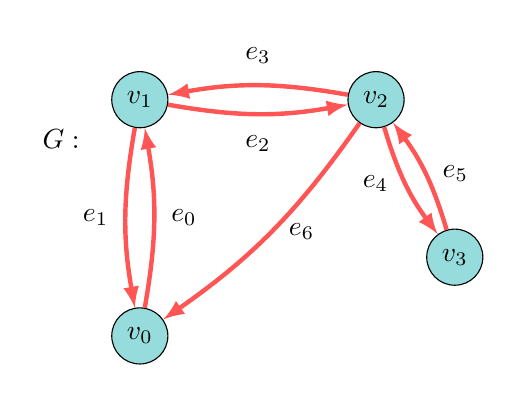
\begin{tikzpicture}
            \definecolor{vertex_color}{RGB}{150,220,220}
            \definecolor{edge_color}{RGB}{255,85,85}
            \tikzstyle{every node} = [draw, fill=vertex_color, shape=circle]
            \tikzstyle{ann} = [draw=none, fill=none, text=black]
            \node (v0) at (0,0) {$v_0$};
            \node (v1) at (0,3) {$v_1$};
            \node (v2) at (3,3) {$v_2$};
            \node (v3) at (4,1) {$v_3$};
            \draw[ultra thick, edge_color,-latex] (v0) edge[bend right=10] node[ann,right] {$e_0$} (v1);
            \draw[ultra thick, edge_color,-latex] (v1) edge[bend right=10] node[ann,left] {$e_1$} (v0);
            \draw[ultra thick, edge_color,-latex] (v1) edge[bend right=10] node[ann,below] {$e_2$} (v2);
            \draw[ultra thick, edge_color,-latex] (v2) edge[bend right=10] node[ann,above] {$e_3$} (v1);
            \draw[ultra thick, edge_color,-latex] (v2) edge[bend right=10] node[ann,left] {$e_4$} (v3);
            \draw[ultra thick, edge_color,-latex] (v3) edge[bend right=10] node[ann,right] {$e_5$} (v2);
            \draw[ultra thick, edge_color,-latex] (v2) edge[bend left=10] node[ann,right] {$e_6$} (v0);
            \node[ann] at (-1,2.5) {$G:$};
        \end{tikzpicture}
        \caption{Vertex-based}
        \label{fig:edge_based_graph_a}
    \end{subfigure}
    \hspace{5mm}
    \begin{subfigure}[Directed]{0.4\linewidth}
        \centering
        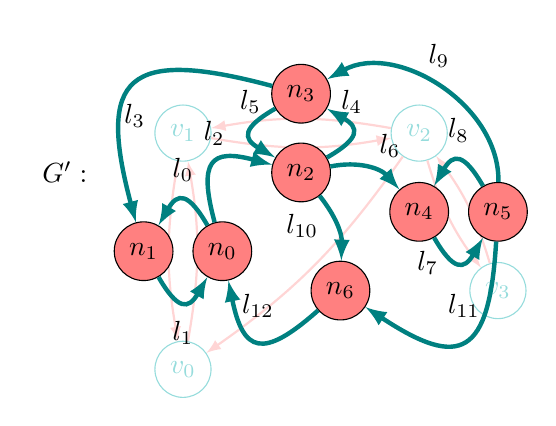
\begin{tikzpicture}
            \definecolor{vertex_color}{RGB}{150,220,220}
            \definecolor{line_color}{RGB}{0,128,128}
            \definecolor{edge_color}{RGB}{255,213,213}
            \definecolor{node_color}{RGB}{255,128,128}
            \tikzstyle{every node} = [draw, fill=node_color, shape=circle]
            \tikzstyle{ann} = [draw=none, fill=none, text=black]
            \node[ann, draw=vertex_color, text=vertex_color] (v0) at (0,0) {$v_0$};
            \node[ann, draw=vertex_color, text=vertex_color] (v1) at (0,3) {$v_1$};
            \node[ann, draw=vertex_color, text=vertex_color] (v2) at (3,3) {$v_2$};
            \node[ann, draw=vertex_color, text=vertex_color] (v3) at (4,1) {$v_3$};
            \draw[thick, edge_color,-latex] (v0) edge[bend right=10] (v1);
            \draw[thick, edge_color,-latex] (v1) edge[bend right=10] (v0);
            \draw[thick, edge_color,-latex] (v1) edge[bend right=10] (v2);
            \draw[thick, edge_color,-latex] (v2) edge[bend right=10] (v1);
            \draw[thick, edge_color,-latex] (v2) edge[bend right=10] (v3);
            \draw[thick, edge_color,-latex] (v3) edge[bend right=10] (v2);
            \draw[thick, edge_color,-latex] (v2) edge[bend left=10] (v0);
            \node (n0) at (0.5, 1.5) {$n_0$};
            \node (n1) at (-0.5, 1.5) {$n_1$};
            \node (n2) at (1.5, 2.5) {$n_2$};
            \node (n3) at (1.5, 3.5) {$n_3$};
            \node (n4) at (3, 2) {$n_4$};
            \node (n5) at (4, 2) {$n_5$};
            \node (n6) at (2, 1) {$n_6$};
            \draw[ultra thick, line_color, -latex] (n0) edge[out=90, in=90, bend right=60, looseness=2] node[ann,above] {$l_0$} (n1);
            \draw[ultra thick, line_color, -latex] (n1) edge[out=270, in=270, bend right=60, looseness=2] node[ann,below] {$l_1$} (n0);
            \draw[ultra thick, line_color, -latex] (n0) edge[out=90, in=280, bend left=60, looseness=2] node[ann,above] {$l_2$} (n2);
            \draw[ultra thick, line_color, -latex] (n3) edge[bend right=60, looseness=2] node[ann,below] {$l_3$} (n1);
            \draw[ultra thick, line_color, -latex] (n2) edge[out=65, in=340, bend right=60, looseness=2] node[ann,above] {$l_4$} (n3);
            \draw[ultra thick, line_color, -latex] (n3) edge[out=200, in=160, bend right=60, looseness=2] node[ann,above] {$l_5$} (n2);
            \draw[ultra thick, line_color, -latex] (n2) edge[out=0, in=120, bend left=30, looseness=1] node[ann,above right] {$l_6$} (n4);
            \draw[ultra thick, line_color, -latex] (n4) edge[out=290, in=270, bend right=60, looseness=2] node[ann,left] {$l_7$} (n5);
            \draw[ultra thick, line_color, -latex] (n5) edge[out=90, in=90, bend right=60, looseness=2] node[ann,above] {$l_8$} (n4);
            \draw[ultra thick, line_color, -latex] (n5) edge[bend right=60, looseness=1] node[ann,above] {$l_9$} (n3);
            \draw[ultra thick, line_color, -latex] (n2) edge[out=300, in=90, bend left=20, looseness=1] node[ann,left] {$l_{10}$} (n6);
            \draw[ultra thick, line_color, -latex] (n5) edge[out=300, in=0, bend left=60, looseness=2] node[ann,above] {$l_{11}$} (n6);
            \draw[ultra thick, line_color, -latex] (n6) edge[out=200, in=300, bend left=60, looseness=2] node[ann,above] {$l_{12}$} (n0);
            \node[ann] at (-1.5,2.5) {$G':$};
        \end{tikzpicture}
        
        \caption{Edge-based}
        \label{fig:edge_based_graph_b}
    \end{subfigure}
    \caption{Transformation of a graph $G$ to an \textit{edge-based} graph $G'$.}
    \label{fig:edge_based_graph}
\end{figure}

As one can see, the complexity and size of the graph grows in the transformation, what was $|V| = 4$ vertices and $|E| = 7$ edges became $|N| = 7$ nodes and $|L| = 13$ lines. The increase in size of the data structures is one drawback with this simple transformation, but on the positive side is the fact that one can apply ordinary algorithms such as Dijkstra to the edge-based graph just as easily as on the original graph. Another disadvantage might be that it lets the topology represent metrics, i.e. a turn restriction is hard coded into the topology, so how does one handle temporary restrictions?

Volker \cite{volker-turncost} has written a study on ``Route Planning with Turn Costs'' and uses edge-based graphs as the foundation. He also introduces an \emph{interface graph} as a link between a vertex-based and an edge-based graph. This new graph builds on an elaboration on what a turn and a junction actually is, with an incoming and an outgoing edge being adjacent on the junction vertex. One can thus see a turn $T$ as either $T = (e_{in}, e_{out})$, i.e. an incoming and an outgoing edge, or as $T = (s,t,u)$ as going from vertex $s$ to vertex $u$, \emph{via} vertex $t$. This kind of finer look at what a turn is, is also used by others to build a more compact representation, see below, section \ref{compact-turn}.

\subsubsection{Turn tables} \label{compact-turn}
One way of dealing with a more compact representation of turns and restrictions and costs associated with them is presented in ``Efficient Routing in Road Networks with Turn Costs'' \cite{geisberger-vetter-turn-cost-2011}, where they use a standard vertex-based graph (where roads are edges and junctions are vertices) on which they use speed-up techniques such as \emph{Contraction Hierarchies}, but they associate each junction with a table that describes the costs of turns there, essentially describing all possible turns and restrictions. It turns out that a lot of junctions in a road map share the same characteristics and therefore can share the same \emph{turn table}, so that on a map over Europe on average 18 vertices could share the same turn table. Thereby they managed to reduce preprocessing time by a factor 3.4 and space by a factor 2.4 with the same query times.

Another solution which uses the vertex-based graph with a turn table at the junctions is described in ``Customizable Route Planning in Road Networks'' \cite[p.6]{crp-2013}. Their solution uses a \emph{separator-based} speed-up technique, which has been viewed as slower than hierarchical techniques, but they argue that this is the most flexible solution with a clean separation of \emph{topology} and \emph{metrics}, with two preprocessing stages before the query stage; one slow \emph{metric-independent} that works on the topology, and a faster \emph{metric customization} stage that can be run for each metric (takes about a second). This solution also uses the fact that many junctions share the same characteristics and therefore turn tables can be shared.


\subsubsection{Bidirectional edges}
So far we have thought of the directed original graph as having an edge for each direction of travel between two vertices, as with edges $e_0$ and $e_1$ in figure \ref{fig:edge_based_graph_a}. But this can be more compactly represented with one edge having a couple of flags indicating directions, meaning that for most roads we need not have two  complete edge structures, but only one with two extra bits indicating the direction. This is however not something that can be done in an edge-based graph as the \emph{lines} in it are not bidirectional.


\section{Map data}
One needs to have good map data as the source for building these data structures and apply smart algorithms on. With poor data it does not matter if one has smart algorithms. A said earlier, a race in route planning started with the public release of previously proprietary data. About the same time \emph{OpenStreetMap} also began, which is an \emph{crowd-sourced} project, meaning that anyone interested can be a cartographer and contribute with map data. Over the years the project has grown to an impressive size, and is used as the base for many applications. However, it turns out that the map data actually lacks a lot of turn restrictions. They might be hard to enter, and they are impossible to spot when comparing aerial photos with maps. Efentakis et al. states that for Athens with 277 thousand vertices only 214 restrictions were entered. They propose an automated remedy by comparing GPS-traces to the maps and deducing that turns seldom made are actually banned and could be marked as restricted in the map data \cite{efentakis-2014}. 

All the same, a lot of high quality applications exists built on \emph{OSM} (OpenStreetMap) data and this project aims at that to.

\subsection{Projections}
Generally speaking, the globe is spherical, but a map is flat. That means that one somehow needs to \textit{project} the spherical data on a flat surface. There exists a lot of different \textit{projections} that tries to do it best. To keep track of which projection one is working in, one can identify it by its \textit{SRID -- Spatial Reference System Identifier} that uniquely identifies which projection and which kind of coordinate system one works with.

\subsection{Topology}
The \textit{topology} is about the relationship between objects in a map \cite{qgis-topology}. If one only thinks of a map as a collection of lines, it is hard to make something out of that information. It becomes useful when we understand the topology, that ``this line is connected to that line at this point''. The we have a relationship between the lines and can understand how to travel on the map.

Analyzing the topology also makes it possible to correct errors made while adding items to the map data, such as if two lines don't actually meet. Then there is a gap and there is no connection. When analyzing, one can opt to connect lines that are within a small distance of one another, thereby correcting mapping errors.

\section{Available applications}\label{sect:available-applications}
Some of the research described earlier in this chapter is used actual working applications. For example \emph{CRP (Customizable Route Planning)} \cite{crp-2013} is used in Bing Maps, and \emph{CH (Contraction Hierarchies)} are used in for example GraphHopper\footnote{\url{https://graphhopper.com/}} and OSRM\footnote{\url{http://project-osrm.org/}}, and they are open source routing applications. So the source code is available so one can study how the data structures are implemented and how the algorithms work. There exists a lot of other solutions built on OSM as well\footnote{\url{http://wiki.openstreetmap.org/wiki/Applications_of_OpenStreetMap}}, using Contraction Hierarchies or other speed-up techniques.

\section{Memory or database}
All research referred to so far has been about building data structures to be held \emph{in memory} so algorithms can operate on them. But as we speak of \emph{queries}, on might think that databases and query languages might be useful as well. There is some research, and a technique called \emph{HLDB} is interesting \cite{hldb-2012}, \cite{hldb-msr-2012}. It is fast enough, and very flexible, permitting to query for \emph{alternative routes} and \emph{points of interest}.

\emph{pgRouting} is an open source database extension to \emph{PostgreSQL}, often used for holding OpenStreetMap-data. It has a function called \verb|pgr_trsp|\footnote{\url{http://docs.pgrouting.org/2.0/en/src/trsp/doc/index.html}} that looks for the shortest path with turn restrictions, so obviously standard relational databases can be part of a solution.

\end{document}